%====================================================================================
\section[Producción]{Producción en la caja de Edgeworth}
%====================================================================================

\begin{frame}
	Las empresas y sus respectivas isocuantas (curvas que determinan el nivel de producción) y la combinación de factores de producción.
		\begin{center}
				\vspace{3cm}
			\hspace{-11cm} \begin{tikzpicture}[transform canvas={scale=0.6}]
	% Formato de CAJA
		\draw[->] (0.5,0.5) node[align=center, below left] {\footnotesize $O_A$} -- (0.5,4.5) node[align=center, above] {\footnotesize $K^{A}$};
		\draw[->] (0.5,0.5) -- (8.5,0.5) node[align=center, right] {\footnotesize $L^{A}$};
	
		% Curvas de indiferencia1
			% Agente B
				\draw  [blue] (0.6,4) ..controls (1.4,1.4) and (1.74,1) .. (6,0.6);
				\draw  [blue] (1,4.3) ..controls (1.7,2.1) and (2,1.6) .. (6.3,1);
				\draw  [blue] (1.6,4.6) ..controls (2.1,3.2) and (1.74,2.2) .. (6.7,1.4);
			
			% Flechas
				\node[draw, single arrow,
						minimum height=30mm, minimum width=1mm,
						single arrow head extend=1.5mm,
						anchor=west, blue, fill=blue, scale=0.5, rotate=50] at (2.7,2.7) {};
	
	% Formato de CAJA rotado
		\draw[->] (18,4) node[align=center, above right] {\footnotesize $O_B$} -- (10,4) node[align=center, left] {\footnotesize $L^{B}$};
		\draw[->] (18,4) -- (18,0) node[align=center, below] {\footnotesize $K^{B}$};
	
		% Curvas de indiferencia1
			% Agente B
				\draw [red] (12,3.9) .. controls (16.76,3.5) and (17.1,3.1) .. (17.9,0.5);
				\draw [red] (11.7,3.5) .. controls (16.5,2.9) and (16.8,2.4) .. (17.3,0.2);
				\draw [red] (11.3,3.1) .. controls (16.76,2.3) and (16.4,1.3) .. (16.6,-0.1);
			
			% Flechas
				\node[draw, single arrow,
						minimum height=30mm, minimum width=1mm,
						single arrow head extend=1.5mm,
						anchor=west, red, fill=red, scale=0.5, rotate=-130] at (15.7,1.8) {};
\end{tikzpicture}
		\end{center}
	Como en el caso de las economías de \textbf{intercambio puro}, podemos utilizar una caja de
	tamaño igual a la dotación agregada de factores.
\end{frame}
%-------------------------------------------------
\begin{frame}
	Decimos que una asignación de factores de producción es eficiente en el sentido de Pareto si no existe otra combinación de factores alternativa que permita aumentar la producción de alguna empresa sin disminuir la producción de alguna otra. Entonces,  \textbf{\emph{la curva de contrato en producción}} nos indica la eficiencia técnica.
		\begin{center}
				\vspace{-0.7cm}
			 \vspace{-0.5cm}
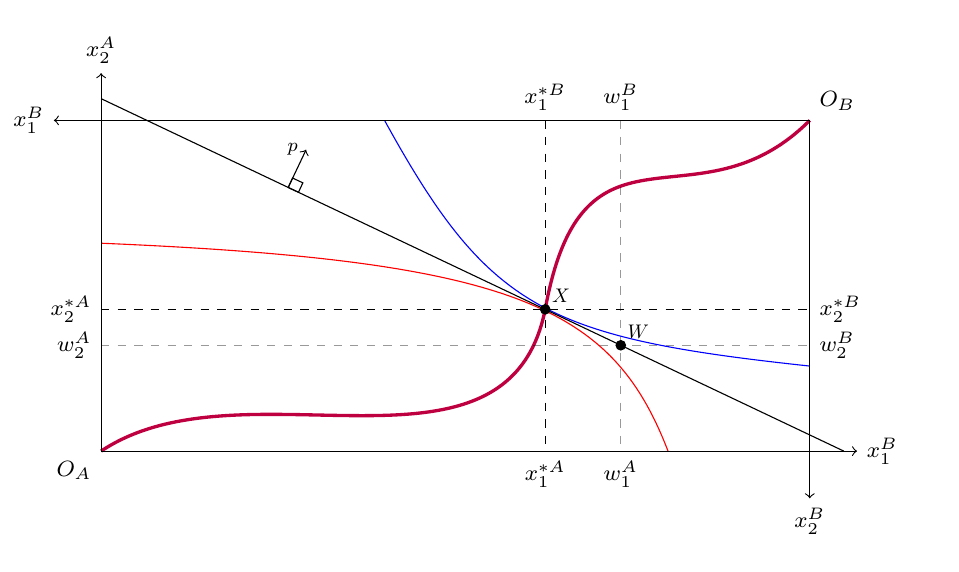
\begin{tikzpicture}[scale=1.2]
	\hspace{-0.3cm}
	% Curva de contrato 5.2,2
		\draw  [purple, very thick] (0.5,0.5) ..controls (2,1.5) and (4.8,0) .. (5.2,2) ..controls (5.6,4.2) and (6.8,2.8) .. (8,4);
	% Intersección de una dotación
		% Demanda: x
			\draw[dashed] (5.2,4) node[above] {\footnotesize $x_{1}^{*B}$} -- (5.2,0.5) node[below]{\footnotesize $x_{1}^{*A}$};
			\draw[dashed] (0.5,2) node[left] {\footnotesize $x_{2}^{*A}$} -- (8,2)node[right]{\footnotesize $x_{2}^{*B}$};
		
		% Oferta: w
			\draw[dashed, opacity=0.4] (6,4) -- (6,0.5);
			\draw[dashed, opacity=0.4] (0.5,1.62)  -- (8,1.62);
			
			\draw (8,1.62)  node [right] {\footnotesize $w_{2}^{B}$};
			\draw (6,4)  node [above] {\footnotesize $w_{1}^{B}$};
			
			\draw (0.5,1.62)  node [left] {\footnotesize $w_{2}^{A}$};
			\draw (6,0.5)  node [below] {\footnotesize $w_{1}^{A}$};
	
	% Curvas de indiferencia
		\draw [blue] (3.5,4) .. controls (4.6,2) and (5.2,1.7) .. (8,1.4);
		\draw [red] (0.5,2.7) .. controls (4.915,2.515) and (5.915,2.015) .. (6.5,0.5);
	
	% Recta presupuestaria
		\draw (0.5,4.23) -- (8.36,0.5);
	
	% Puntos
		\draw[black, fill=black] (5.2,2) circle[radius=0.05] node [above right, scale=0.25mm] {$X$};
		\draw[black, fill=black] (6,1.62) circle[radius=0.05] node [above right, scale=0.25mm] {$W$};
	
	% Flecha y rectángulo
		\draw [->] (2.48,3.29) -- (2.67,3.69) node [left, scale = 0.3mm] {\footnotesize $p$};
		\draw [rotate around={-25:(2.48,3.29)}] (2.48,3.29) rectangle (2.6, 3.4);
		
	% Formación de la caja
		% Consumidor A
			\draw[->] (0.5,0.5) node[align=center, below left] {\footnotesize $O_A$} -- (0.5,4.5) node[align=center, above] {\footnotesize $x_{2}^{A}$};
			\draw[->] (0.5,0.5) -- (8.5,0.5) node[align=center, right] {\footnotesize $x_{1}^{B}$};
		
		%Consumidor B
			\draw[->] (8,4) node[align=center, above right] {\footnotesize $O_B$} -- (0,4) node[align=center, left] {\footnotesize $x_{1}^{B}$};
			\draw[->] (8,4) -- (8,0) node[align=center, below] {\footnotesize $x_{2}^{B}$};
\end{tikzpicture}
		\end{center}
\end{frame}
%-------------------------------------------------
\begin{frame}
	La relación gráfica anterior está representada por la siguiente expresión matemática
		\begin{align*}
			& \text{Max } \quad Q^{A}\left(L^{A},K^{A}\right) \\
			& \begin{array}{ll}
				\text{s.a: } & Q^{B}\left(L^{B},K^{B} \right) = \overline{Q}^{B}\\
							 & L^{A}+L^{B} = \overline{L}  \\
							 & K^{A}+K^{B} = \overline{K}  
			\end{array}
		\end{align*}
	Cuyo resultado final es la condición de eficiencia:
		$$RMST^A = RMST^B$$
	\textbf{Eficiencia en el uso de los factores de producción o , simplemente, eficiencia técnica}
\end{frame}
%-------------------------------------------------
\begin{frame}
	Las empresas pueden alcanzar asignaciones de factores productivos eficientes a partir del libre funcionamiento de los mercados perfectamente competitivos; es decir, con la \textbf{introducción de precios} (precio de los factores de producción).
	\begin{center}
		\begin{tikzpicture}[scale=1]
	% Formación de la caja
	% Consumidor A
	\draw[->] (0.5,0.5) node[align=center, below left] {\footnotesize $O_A$} -- (0.5,4.5) node[align=center, above] {\footnotesize $x_{2}^{A}$};
	\draw[->] (0.5,0.5) -- (8.5,0.5) node[align=center, right] {\footnotesize $x_{1}^{A}$};
	
	\draw (6,0.5) node[below] {\footnotesize $x_{1}^{A}$};
	\draw (0.5,2) node[left] {\footnotesize $x_{2}^{A}$};
	
	% Llaves
	\draw [decorate,decoration={brace,amplitude=5pt},xshift=-4pt,yshift=0pt] (6.1,-0.05) -- (0.7,-0.05);
	\node [right] at (3,-0.4) {$w_{1}^{A}$};
	
	\draw [decorate,decoration={brace,amplitude=5pt},xshift=-4pt,yshift=0pt] (-0.05,0.5) --(-0.05,2);
	\node [left] at (-0.3,1.27) {$w_{2}^{A}$};
\end{tikzpicture}
	\end{center}
\end{frame}
%-------------------------------------------------
\begin{frame}
	La introducción de precios conlleva a que las empresas busquen maximizar  beneficio $\pi$ o minimizando costos, entonces por dualidad:
		$$
			\begin{array}{ccc}
				\text{Max } pQ(L,K) - wL - rK & {} & \text{Min } wL + rK\\[0.3cm]
				\text{s.a: } wL + rK = \overline{CT}& {} & \text{s.a: } Q(L,K) = \overline{Q}
			\end{array}
		$$
	Cuyo resultado final muestra la eficiencia técnica para ambas empresas con la incorporación de precios:
		$$RMST^A = RMST^B = \frac{w}{r}$$
\end{frame}